\documentclass[10pt,twocolumn]{article}
\usepackage[margin=0.8in]{geometry}
\usepackage{amsmath,amssymb,booktabs,graphicx,xcolor}
\usepackage{pgfplots}
\pgfplotsset{compat=1.17}
\usepackage[hidelinks]{hyperref}
\usepackage{caption}
\captionsetup{font=small,labelfont=bf}
% Generated by generate_tables.py -- do not edit by hand.
\newcommand{\ArmRows}{C1 & star & free (SABRE) & 3 & 163 & 213 & 0.0160 (0.0019) & 0.0171 & 0.0256 & 6.7\\
C2 & star & best path & 3 & 79 & 91 & 0.0723 (0.0073) & 0.2594 & 0.0748 & 12.2\\
C3 & star & best path & 1 & 147 & 179 & 0.0927 (0.0088) & 0.1072 & 0.1286 & 12.2\\
C4 & chain & best path & 1 & 39 & 86 & 0.2173 (0.0095) & 0.4048 & 0.2475 & 12.2\\
C5 & chain & best path & 3 & 39 & 66 & 0.2150 (0.0055) & 0.4054 & 0.2381 & 12.2\\
C6 & chain & median path & 3 & 39 & 66 & 0.1096 (0.0048) & 0.2783 & 0.1246 & 22.3\\
C7 & chain & free (level-3 default) & 3 & 39 & 66 & 0.1580 (0.0085) & 0.4404 & 0.1716 & 22.3\\}
\newcommand{\ContrastRows}{C5$-$C2 & rewrite + SWAP removal, opt.\ 3 & +14.27 & [+13.52, +15.01] & $4.6\times10^{-11}$ & $9.8\times10^{-3}$ & +16.32 & $1.8\times10^{-11}$\\
C4$-$C3 & rewrite + SWAP removal, opt.\ 1 & +12.47 & [+11.52, +13.42] & $8.4\times10^{-10}$ & $9.8\times10^{-3}$ & +11.88 & $1.5\times10^{-10}$\\
C5$-$C6 & best vs median path, 39 CZ & +10.54 & [+9.95, +11.12] & $6.2\times10^{-11}$ & $9.8\times10^{-3}$ & +11.35 & $4.1\times10^{-11}$\\
C5$-$C4 & virtual-$Z$ A/A control & -0.24 & [-0.88, +0.41] & 0.43 & 0.32 & -0.94 & 0.04\\
C5$-$C7 & greedy best path vs stock layout & +5.70 & [+5.13, +6.28] & $6.6\times10^{-9}$ & $9.8\times10^{-3}$ & +6.65 & $7.1\times10^{-10}$\\}
\newcommand{\ObsCoords}{(C1,0.0160) +- (0,0.0019) (C2,0.0723) +- (0,0.0073) (C3,0.0927) +- (0,0.0088) (C4,0.2173) +- (0,0.0095) (C5,0.2150) +- (0,0.0055) (C6,0.1096) +- (0,0.0048) (C7,0.1580) +- (0,0.0085)}
\newcommand{\PredCoords}{(C1,0.0171) (C2,0.2594) (C3,0.1072) (C4,0.4048) (C5,0.4054) (C6,0.2783) (C7,0.4404)}
\newcommand{\BlockDiffCoords}{(0.865,14.423) (0.895,14.408) (0.925,14.470) (0.955,11.907) (0.985,14.460) (1.015,13.068) (1.045,15.322) (1.075,14.393) (1.105,14.968) (1.135,15.267) (1.865,11.252) (1.895,13.347) (1.925,9.856) (1.955,12.448) (1.985,12.818) (2.015,13.510) (2.045,12.405) (2.075,11.503) (2.105,12.944) (2.135,14.591) (2.865,10.194) (2.895,11.414) (2.925,10.215) (2.955,8.649) (2.985,11.218) (3.015,10.222) (3.045,10.605) (3.075,11.393) (3.105,10.855) (3.135,10.597) (3.865,0.463) (3.895,-0.557) (3.925,1.650) (3.955,-1.172) (3.985,-0.964) (4.015,-0.467) (4.045,-1.065) (4.075,0.009) (4.105,0.542) (4.135,-0.794) (4.865,4.756) (4.895,5.143) (4.925,6.668) (4.955,4.795) (4.985,6.303) (5.015,5.791) (5.045,5.438) (5.075,7.022) (5.105,4.993) (5.135,6.112)}
\newcommand{\JobId}{dbto408n26qs739tnrj0}
\newcommand{\Blocks}{10}
\newcommand{\Shots}{2{,}048}
\newcommand{\TotalShots}{184{,}320}
\newcommand{\NPubs}{90}
\newcommand{\UnionQubits}{96}
\newcommand{\UnionReadout}{2.47}
\newcommand{\QFortyTwo}{22.3}
\newcommand{\QFortyOne}{12.1}
\newcommand{\QThirtyOne}{12.2}
\newcommand{\NPaths}{400}
\newcommand{\LockSha}{5f4a04c45933e046c0fff0574a426fd3a876ec5f19d808d69514374c2f931f1f}
\newcommand{\QpySha}{409dc7365405ed20bde035683ae022a09778a1c58e186edd64fe5077154d7bf9}
\newcommand{\QpuSeconds}{53}


\title{\bfseries Same gate count, half the fidelity: a preregistered decomposition of layout,
routing and optimisation-level effects on a 40-qubit circuit on \texttt{ibm\_marrakesh}}
\author{Devin Phillip Davis\\ \small Agile Defense Systems LLC}
\date{20 November 2026 \quad (TESSERACT-MAP-02 results, version 1.0)}

\begin{document}
\maketitle

\begin{abstract}
\noindent
We ran a preregistered, blocked hardware experiment that separates four compilation factors that an
earlier, unplanned rerun of a 40-qubit circuit had changed all at once: the logical structure of the
circuit (a degree-20 CNOT star or an equivalent degree-2 chain), the choice of physical qubits, SWAP
routing, and the Qiskit optimisation level. Seven arms and two readout-calibration circuits were
interleaved in \Blocks{} randomised blocks of \Shots{} shots on the 156-qubit IBM Heron~r2 processor
\texttt{ibm\_marrakesh} (one job, \TotalShots{} shots, \QpuSeconds{}\,s of QPU time). The primary
endpoint is the classical (Bhattacharyya) fidelity $F_{\mathrm{cl}}$ to the exact four-string output
distribution. Rewriting the star into a chain and removing all SWAPs on the same 40 qubits raised
$F_{\mathrm{cl}}$ by $+14.3$\,pp (optimisation level~3) and $+12.5$\,pp (level~1). At a fixed 39~CZ
gates and depth~66, moving the circuit from a calibration-ranked best path to a median path cost
$10.5$\,pp, halving the fidelity. A greedy calibration-weighted path beat Qiskit's stock level-3
layout by $5.7$\,pp, the reverse of what a \texttt{FakeMarrakesh} noise-model simulation predicted
before the run. A built-in virtual-$Z$ A/A control was null ($-0.24$\,pp, 95\% CI $[-0.88,+0.41]$).
All four effect contrasts survive Holm correction ($p_{\mathrm{Holm}}\le 6.6\times10^{-9}$) and an
exact Wilcoxon check. Union readout calibration found assignment errors of \QFortyTwo\% and
\QFortyOne\% on two qubits that IBM's calibration listed near 1\%; both lie on the losing layouts.
The noise-model simulation overestimated every structured arm by roughly a factor of two. These
are compilation and device-heterogeneity effects from one job on one device; we make no claim beyond
that.
\end{abstract}

\section{Background}
A 40-qubit ``tesseract'' circuit from this project was originally reported with an implausible
error-suppression figure, later withdrawn~\cite{erratum}. An archived rerun on \texttt{ibm\_kingston}
(job \texttt{dansntf8gn2s739n32e0}) found the four-string ideal support rose from 5.3\% to 18.0\% when
the circuit was rewritten and remapped, but that rerun changed four factors at once and saved no
layouts, so no single cause could be identified. TESSERACT-MAP-02 was designed to separate them.

The logical circuit prepares, from two seed qubits rotated by $\theta=51.7^\circ$, the state whose
ideal output has support on exactly four 40-bit strings
$\mathcal{S}_4=\{0^{40},1^{40},(10)^{20},(01)^{20}\}$ with probabilities
$\tfrac12\cos^2\theta,\tfrac12\cos^2\theta,\tfrac12\sin^2\theta,\tfrac12\sin^2\theta$. In the
\emph{star} form every even wire is a CNOT target of qubit~0 and every odd wire of qubit~1 (hub
degree~20); in the \emph{chain} form each wire copies its neighbour two places back (degree~2). The
two forms are exactly equivalent (statevector overlap 1 to $10^{-15}$ at $N=12$; GF(2) propagation
at $N=40$). A star of degree~20 cannot embed in heavy-hex (maximum degree~3), so the star always
needs SWAPs, while the chain embeds in a 40-qubit simple path with none.

\section{Design}
\paragraph{Arms.} Seven arms (Table~\ref{tab:arms}) vary one or two factors at a time. C1 is the
original circuit with free layout and SABRE routing. C2/C3 pin the star to the best path and let
SABRE route it at optimisation levels 3/1. C4/C5 run the chain on the best path with no routing at
levels 1/3. C6 runs the chain on the median-cost path. C7 hands the chain to Qiskit's level-3 layout
pipeline with no pinned qubits. Two circuits per block prepare $|0\rangle^{\otimes}$ and
$|1\rangle^{\otimes}$ on all \UnionQubits{} qubits used by any arm (union readout calibration).

\paragraph{Path selection.} \NPaths{} candidate 40-qubit simple paths were scored on the
calibration snapshot taken at lock time (sum of CZ, readout and decoherence error terms); the best
and median paths were frozen before submission, so the evaluation data played no part in choosing
them.

\paragraph{Contrasts.} Five contrasts were preregistered:
(1) C5$-$C2 and (2) C4$-$C3, the logical rewrite plus SWAP removal on identical qubits;
(3) C5$-$C6, physical path quality at a fixed 39~CZ, depth~66 and level~3;
(4) C5$-$C4, an A/A control: the two arms have the same \texttt{sx} and \texttt{cz} counts (81, 39)
and differ only by 40 zero-duration virtual \texttt{rz} gates, so the expected difference is zero;
(5) C5$-$C7, greedy best path against the stock layout pipeline.

\paragraph{Statistics.} The block is the unit of replication; shots are never treated as
independent replicates. Each contrast is a two-sided paired $t$-test over the \Blocks{} blocks
(df~$=9$), with Holm--Bonferroni correction across the five at family-wise $\alpha=0.05$. An exact
Wilcoxon signed-rank test was preregistered as a sensitivity check. The secondary endpoint is the
probability mass on $\mathcal{S}_4$, $P(\mathcal{S}_4)$.

\paragraph{Preregistration and amendment.} The design, endpoints and decision matrix were written
and simulated before any hardware access. Amendment A-1 (recorded before the job) cut the size
from 15 blocks $\times$ 4{,}096 shots to \Blocks{} $\times$ \Shots{} to fit the IBM Open Plan quota,
lowering the 85\%-power minimum detectable effect from 1.5 to about 2.3\,pp. The lock file
(SHA-256 \texttt{\detokenize{5f4a04c4...}}) and compiled QPY (\texttt{\detokenize{409dc736...}}) were
pushed to a public repository before the job was submitted; full hashes are in the data record.

\section{Results}
The job (\texttt{\JobId}) ran \NPubs{} PUBs in about 66\,s of wall-clock time on 16 November 2026.
Observed paired block-difference SDs were 0.008--0.013, smaller than the 0.0165 assumed in A-1, and
every 95\% confidence half-width is below 1\,pp, so the reduced size did not limit any conclusion.

\begin{table*}[t]
\centering\footnotesize\setlength{\tabcolsep}{4pt}
\caption{Arms. $F_{\mathrm{cl}}$ is the mean over \Blocks{} blocks (SD across blocks). ``Predicted''
is the \texttt{FakeMarrakesh} surrogate simulation made before the run. ``Max RO'' is the largest
union-calibration readout assignment error among the arm's 40 qubits.}
\label{tab:arms}
\begin{tabular}{@{}lllrrrlrrr@{}}
\toprule
Arm & Logical & Layout & Opt & CZ & Depth & $F_{\mathrm{cl}}$ (SD) & Predicted & $P(\mathcal{S}_4)$ & Max RO (\%)\\
\midrule
\ArmRows
\bottomrule
\end{tabular}
\end{table*}

\begin{table*}[t]
\centering\small
\caption{Preregistered paired contrasts, in percentage points of $F_{\mathrm{cl}}$ (primary) and
$P(\mathcal{S}_4)$ (secondary). Holm-adjusted $p$ values across the five contrasts. With
$n=10$ blocks the smallest attainable Holm-adjusted exact Wilcoxon $p$ is $9.8\times10^{-3}$; four
contrasts reach it (every block favoured the same arm).}
\label{tab:contrasts}
\footnotesize\setlength{\tabcolsep}{4pt}
\begin{tabular}{@{}llrcrrrr@{}}
\toprule
& & \multicolumn{4}{c}{Primary: $F_{\mathrm{cl}}$} & \multicolumn{2}{c}{Secondary: $P(\mathcal{S}_4)$}\\
\cmidrule(lr){3-6}\cmidrule(l){7-8}
Contrast & Factor & $\Delta$ (pp) & 95\% CI (pp) & Holm $p$ & Wilcoxon $p$ & $\Delta$ (pp) & Holm $p$\\
\midrule
\ContrastRows
\bottomrule
\end{tabular}
\end{table*}

\begin{figure}[t]
\centering
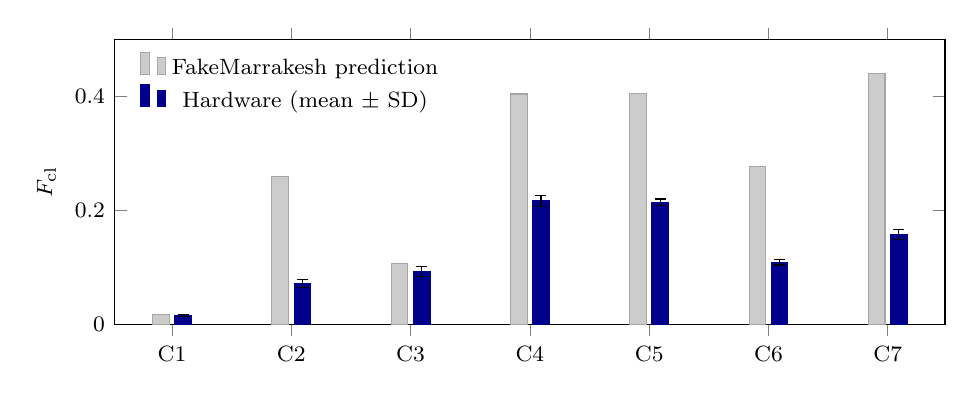
\begin{tikzpicture}
\begin{axis}[width=\columnwidth,height=5.2cm,ybar,bar width=6pt,
  symbolic x coords={C1,C2,C3,C4,C5,C6,C7},xtick=data,ymin=0,ymax=0.5,
  ylabel={$F_{\mathrm{cl}}$},legend style={at={(0.02,0.98)},anchor=north west,font=\footnotesize,draw=none},
  tick label style={font=\footnotesize},label style={font=\footnotesize},enlarge x limits=0.08]
\addplot+[fill=gray!40,draw=gray!70] coordinates {\PredCoords};
\addplot+[fill=blue!55!black,draw=blue!55!black,error bars/.cd,y dir=both,y explicit,error bar style={black}] coordinates {\ObsCoords};
\legend{FakeMarrakesh prediction,Hardware (mean $\pm$ SD)}
\end{axis}
\end{tikzpicture}
\caption{Predicted versus observed $F_{\mathrm{cl}}$. The surrogate was close only for the
worst arm (C1) and inverted two orderings: C2/C3 and C5/C7.}
\label{fig:pred}
\end{figure}

\begin{figure}[t]
\centering
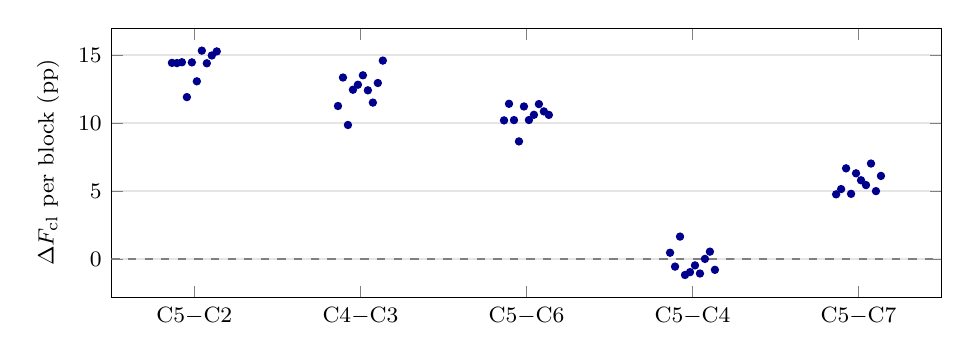
\begin{tikzpicture}
\begin{axis}[width=\columnwidth,height=5cm,xmin=0.5,xmax=5.5,
  xtick={1,2,3,4,5},xticklabels={C5$-$C2,C4$-$C3,C5$-$C6,C5$-$C4,C5$-$C7},
  ylabel={$\Delta F_{\mathrm{cl}}$ per block (pp)},tick label style={font=\footnotesize},
  label style={font=\footnotesize},ymajorgrids,grid style={gray!20}]
\addplot[only marks,mark=*,mark size=1.3pt,blue!55!black] coordinates {\BlockDiffCoords};
\addplot[gray,dashed,domain=0.5:5.5] {0};
\end{axis}
\end{tikzpicture}
\caption{Per-block paired differences for the five contrasts (10 blocks each, jittered
horizontally). Only the A/A control (C5$-$C4) straddles zero.}
\label{fig:blocks}
\end{figure}

\paragraph{Rewrite and SWAP removal.} On the same 40 physical qubits, the chain with no SWAPs beat
the routed star by $+14.27$\,pp at level~3 (79$\to$39 CZ) and $+12.47$\,pp at level~1 (147$\to$39 CZ).
This combines fewer CZ gates, lower depth and the change of logical structure; the design does not
separate them.

\paragraph{Physical path quality.} At identical CZ count, depth and optimisation level, the best path
(C5, $F_{\mathrm{cl}}=0.215$) beat the median path (C6, $0.110$) by $+10.54$\,pp
(95\% CI $[+9.95,+11.12]$) and won in all 10 blocks. Qubit choice alone roughly halves the fidelity of
this circuit.

\paragraph{Greedy path versus the stock layout.} C5 beat C7 by $+5.70$\,pp. Before the run, the
surrogate simulation predicted the opposite ($0.440$ for C7 against $0.405$ for C5), and the
preregistered decision row ``C7 $\ge$ C5 $\gg$ C1'' is therefore not met.

\paragraph{A/A control.} C5$-$C4 is $-0.24$\,pp (95\% CI $[-0.88,+0.41]$, Holm $p=0.43$), ruling out
residual within-block drift or single-qubit-layer effects larger than about 0.9\,pp on the primary
endpoint. On the secondary endpoint the same contrast is $-0.94$\,pp (Holm $p=0.038$), below the
preregistered 1.5\,pp decision threshold and opposite in sign to the hypothesis that compressing
single-qubit layers helps. We did not re-check against the backend that the two arms share one
physical pulse schedule, so we report this as an unexplained small difference.

\paragraph{Readout outliers.} Union calibration over \UnionQubits{} qubits gave a mean assignment
error of \UnionReadout\%. Three qubits stood out: q42 (\QFortyTwo\%), q41 (\QFortyOne\%) and q31
(\QThirtyOne\%). IBM's reported readout errors for q41 and q42 were 1.0--1.3\% in both the lock-time
and execution-time snapshots. q41 and q42 lie on the median path (C6) and on the stock layout (C7),
not on the best path; q31 lies on the best path and on the median path. Readout on these qubits can
therefore explain part of the C5$-$C6 and C5$-$C7 gaps, but not all of them, and this experiment does
not measure how much. We applied no readout mitigation to the primary endpoint.

\paragraph{Surrogate accuracy.} The \texttt{FakeMarrakesh} surrogate (a calibrated gate, idle
$T_1/T_2$ and domain-wall model, not a full 40-qubit density-matrix simulation) predicted roughly
twice the observed fidelity for every structured arm (C5: 0.405 predicted, 0.215 observed), was
accurate only for C1, and inverted the C2/C3 and C5/C7 orderings. C2 (level~3, 79~CZ) scored below
C3 (level~1, 147~CZ) in all 10 blocks.

\section{Discussion}
For this circuit family on this device, the largest controllable effects are in the order the
compiler normally treats as secondary: which 40 qubits are used (about 10\,pp at fixed gate count)
and whether the circuit is rewritten so that it needs no SWAPs (12--14\,pp). Optimisation level made
no measurable difference on an already SWAP-free chain, and on the routed star level~3 removed 68 CZ
gates yet scored lower than level~1.

The C5/C7 reversal and the surrogate's misranking have a common candidate cause: layout scoring
that relies on reported calibration data misses errors that are not in it, such as the readout
outliers above. Error-aware layout scoring of this kind is standard practice~\cite{nation2023}; our
result is one hardware instance in which it underperformed a greedy alternative by 5.7\,pp, not a
general ranking of layout methods.

\paragraph{Limitations.} One job on one device in one calibration window. No interaction contrast
was run, so additivity of the rewrite and path effects is untested. C5$-$C2 and C4$-$C3 bundle gate
count, depth and logical structure. The readout contribution to the path gaps is not quantified.
The C7 layout was chosen by Qiskit's level-3 pipeline; we did not record which internal pass
produced it. None of these results bear on non-local or exotic physics; they are compilation and
device-heterogeneity effects.

\paragraph{Follow-up.} A natural next experiment adds the missing star/median-path cell (a
$2\times2$ test of additivity), readout-mitigated copies of the best- and median-path arms to
estimate the readout share of the 10.5\,pp gap, and a replication on a second Heron~r2 device.

\section*{Data and code availability}
The accompanying record contains the preregistration, amendment A-1, the lock file, the compiled QPY,
the pre-lock calibration snapshot, the raw counts for all \NPubs{} PUBs, the analysis output, the
Wilcoxon supplement and the scripts that produce every table and figure here
(\texttt{generate\_tables.py}), with a SHA-256 manifest. Two IBM Cloud account identifiers were removed
from the raw-counts file; no count was changed. Source repository:
\url{https://github.com/quantum-osiris/osiris-cli} (\texttt{docs/phase3/}, \texttt{phase2/tesseract\_map\_02/}).

\section*{Acknowledgements}
We acknowledge the use of IBM Quantum services; the views expressed are the author's and do not
reflect the official policy or position of IBM or the IBM Quantum team. Analysis code and this
manuscript were prepared with the assistance of AI coding tools under the author's direction and
review.

\begin{thebibliography}{9}\small
\bibitem{erratum} D.~P.~Davis, OSIRIS ERRATA v2 (2026-09-20), withdrawal of the 40-qubit
``$10^6\times$ error suppression'' figure, originally recorded in Zenodo \texttt{10.5281/zenodo.22870279}.
\bibitem{nation2023} P.~D.~Nation and M.~Treinish, ``Suppressing quantum circuit errors due to system
variability,'' \emph{PRX Quantum} \textbf{4}, 010327 (2023).
\end{thebibliography}
\end{document}
